%SOP Template 
% Version 02 Added revision date
% Version 03 Added TOC and acknowledgements
%           New SOP3_alpha.cls


\documentclass[12pt]{../SOP4_alpha}\usepackage[]{graphicx}\usepackage[]{color}
% maxwidth is the original width if it is less than linewidth
% otherwise use linewidth (to make sure the graphics do not exceed the margin)
\makeatletter
\def\maxwidth{ %
  \ifdim\Gin@nat@width>\linewidth
    \linewidth
  \else
    \Gin@nat@width
  \fi
}
\makeatother

\definecolor{fgcolor}{rgb}{0.345, 0.345, 0.345}
\makeatletter
\@ifundefined{AddToHook}{}{\AddToHook{package/xcolor/after}{\definecolor{fgcolor}{rgb}{0.345, 0.345, 0.345}}}
\makeatother
\newcommand{\hlnum}[1]{\textcolor[rgb]{0.686,0.059,0.569}{#1}}%
\newcommand{\hlstr}[1]{\textcolor[rgb]{0.192,0.494,0.8}{#1}}%
\newcommand{\hlcom}[1]{\textcolor[rgb]{0.678,0.584,0.686}{\textit{#1}}}%
\newcommand{\hlopt}[1]{\textcolor[rgb]{0,0,0}{#1}}%
\newcommand{\hlstd}[1]{\textcolor[rgb]{0.345,0.345,0.345}{#1}}%
\newcommand{\hlkwa}[1]{\textcolor[rgb]{0.161,0.373,0.58}{\textbf{#1}}}%
\newcommand{\hlkwb}[1]{\textcolor[rgb]{0.69,0.353,0.396}{#1}}%
\newcommand{\hlkwc}[1]{\textcolor[rgb]{0.333,0.667,0.333}{#1}}%
\newcommand{\hlkwd}[1]{\textcolor[rgb]{0.737,0.353,0.396}{\textbf{#1}}}%
\let\hlipl\hlkwb

\usepackage{framed}
\makeatletter
\newenvironment{kframe}{%
 \def\at@end@of@kframe{}%
 \ifinner\ifhmode%
  \def\at@end@of@kframe{\end{minipage}}%
  \begin{minipage}{\columnwidth}%
 \fi\fi%
 \def\FrameCommand##1{\hskip\@totalleftmargin \hskip-\fboxsep
 \colorbox{shadecolor}{##1}\hskip-\fboxsep
     % There is no \\@totalrightmargin, so:
     \hskip-\linewidth \hskip-\@totalleftmargin \hskip\columnwidth}%
 \MakeFramed {\advance\hsize-\width
   \@totalleftmargin\z@ \linewidth\hsize
   \@setminipage}}%
 {\par\unskip\endMakeFramed%
 \at@end@of@kframe}
\makeatother

\definecolor{shadecolor}{rgb}{.97, .97, .97}
\definecolor{messagecolor}{rgb}{0, 0, 0}
\definecolor{warningcolor}{rgb}{1, 0, 1}
\definecolor{errorcolor}{rgb}{1, 0, 0}
\makeatletter
\@ifundefined{AddToHook}{}{\AddToHook{package/xcolor/after}{
\definecolor{shadecolor}{rgb}{.97, .97, .97}
\definecolor{messagecolor}{rgb}{0, 0, 0}
\definecolor{warningcolor}{rgb}{1, 0, 1}
\definecolor{errorcolor}{rgb}{1, 0, 0}
}}
\makeatother
\newenvironment{knitrout}{}{} % an empty environment to be redefined in TeX

\usepackage{alltt}

\usepackage[english]{babel}


\title{IDEXX Quanti-Tray DRAFT!}
\date{6/12/2022}
\author{Marc Los Huetos}
\approved{TBD}
\ReviseDate{\today}
\SOPno{23.02}
\IfFileExists{upquote.sty}{\usepackage{upquote}}{}
\begin{document}


\maketitle

\section{Scope and Application}

\NP This standard operating procedure describes the test method for the collection and analysis of water samples for the enumeration of Escherichia coli (E. coli) and
Total coliform bacteria.

\NP The applications of this SOP are for...

\section{Summary of Method}

\NP Surface water samples are collected in 120ml shrink-banded, sterile IDEXX bottles. An undiluted water sample will be analyzed from the sample collected.
The Colilert® reagent is added directly to the 100 ml undiluted sample. Both are mixed thoroughly to dissolve the reagent. The sample is transferred to QuantiTrays®/2000 and sealed using the Quanti-Tray sealer. Samples are incubated at 35.0 ± 0.5º C for 24 hours. Results are reported as MPN/100mL. 

\NP The detection limit for this analysis is 1 Most Probable Number (MPN) per 100mL of sample. 

\tableofcontents

\newpage

\section{Acknowledgements}

\section{Definitions}

\NP Analytical batch: The set of samples processed at the same time

\NP Control cultures: For each lot of medium, check analytical procedures by
testing with known positive and negative control cultures. For example,
E.coli is a positive control for this analysis and Staphylococcus aureus is a
negative control.

\NP Field duplicate (FD): Two samples taken at the same time and place under
identical circumstances and that are treated identically throughout field
and laboratory procedures. Analysis of field duplicates indicates the
precision associated with sample collection, preservation, and storage as
well as laboratory procedures.

\NP Laboratory reagent blank (LRB): An aliquot of sterilized water treated as a
sample in all aspects, except that it is not taken to the sampling site. The
purpose is to determine if the analytes or interferences are present in the
laboratory environment, the reagents, or the apparatus.

\NP Laboratory duplicate (LD): Two aliquots of the same environmental sample
treated identically throughout a laboratory analytical procedure. Analysis
of laboratory duplicates indicates precision associated with laboratory
procedures but not with sample collection, preservation or storage
procedures. 


\section{Biases and Interferences}

\NP Water samples containing humic or other material may be colored. If there is
background color, compare inoculated trays to a control tray containing only
water (SM, 9223 A.) 

\section{Health and Safety}

\NP The analysis involves handling of freshwater samples that may contain live
microorganisms and therefore pose some threat of infection. Laboratory personnel
who are routinely exposed to such water samples are encouraged to protect
themselves from water borne illnesses by wearing clean disposable gloves and
washing their hands frequently.

\NP The Colilert® reagent is not hazardous according to the manufacturer’s material
safety data sheet. The manufacturer does recommend wearing gloves and safety
glasses while using this reagent and washing hands after use. 


\subsection{Safety and Personnnel Protective Equipment}

Water quality can range from high quality and even potoble to very low with assorted pathogens or even toxicty. Thus, it's important to take every precuation possible to protect yourself. 

\section{Personnel \& Training Responsibilities}

\NP Laboratory and field personnel shall have a working knowledge of this analytical procedure and will have received training from a faculty, staff, or student knowledgeable of the proper sample analysis procedures. 

\NP Researchers training is required before this the procedures in this method can be used.

\NP Researchers using this SOP should be trained for the following SOPs:

\begin{itemize}
  \item SOP01 Laboratory Safety
  \item SOP02 Field Safety
  \item SOP23 IDEXX Quanti-Tray
\end{itemize}

\section{Required Materials and Apparati}

\NP 10.1 Sterile, shrink-wrapped 100ml IDEXX bottles.

\NP Quanti-Tray Sealer®: catalog number XXXX? . IDEXX Laboratories, Inc., Westbrook, ME (NEED TO ADD SERIAL NUMBER).

\NP Incubator (add model and serial number) 


\section{Reagents and Standards}

\NP... need to add

?? Colilert® reagent: for 100 ml samples, catalog number WP200. IDEXX Laboratories, Inc., Westbrook, ME.

\NP ?? Quanti-Tray®/2000: 100 trays containing 97 wells each, part number WQT2K. IDEXX Laboratories, Inc., Westbrook, ME

\section{Estimated Time}

\NP This procedure requires XX minutes...

\section{Sample Collection, Preservation, and Storage}

\section{Procedure}

NEEDS TO BE UPDATED!!! copied from various methods online... needs to be harmonized.

a) Good laboratory practices will be used for this procedure.

b) Pre-heat incubator to bring temperature up to 35ºC.

c) Pre-warm rehydration fluid vials to 35º-37ºC. Use blue autoclavable foam vial
holder to hold vials.

d) Discard blue cap from rehydration fluid vial.

e) Remove organism vial from pouch (vial with colorless cap).

f) Transfer colorless cap onto pre-warmed rehydration vial and discard vial
containing the desiccant.

g) Place rehydration vials into the foam vial holder. Invert and place in incubator for
10 minutes at 35º-37ºC.

h) Fill four sterile IDEXX 100 ml. bottles with distilled water to fill line. Label
three bottles with each bacteria name and one bottle “control”. Place in incubator
until a temperature of 35º ± 0.5ºC is reached.

i) Remove vial from holder. Hold vial upside down and tap cap gently to mix.
Remove cap and look at inside surface to ensure that no un-dissolved black
particles are present. Inoculate an additional 10 minutes if present.

j) Add entire contents of each appropriate bacteria vial to pre-warmed 100 ml.
labeled bottles.

k) Add Colilert reagent to sample bottles including control. Place in incubator and
follow incubation instructions outlined in section 7. Do not place in QuantiTrays. 

The 100ml duplicate water sample is shaken well just prior to
preparation for analysis. Samples over the 100 ml mark must not be
poured to volume. If there is at least 1” of headspace, the sample
may be shaken and excess volume taken out with a sterile pipet. If
there is insufficient headspace (<1”) for proper mixing, do not pour
off and discard a portion of the sample. Rather, pour the entire
sample into a larger sterile container, mix properly, and proceed with
the analysis.

Open a Colilert ampule and pour contents into either the diluted
sample or undiluted sample. Repeat for the remaining sample.

Mix thoroughly, making sure the Colilert reagent is completely
dissolved.

Follow manufacturer’s instructions for preparation of QuantiTray/2000 and use of the Quanti-Tray Sealer.

Allow bubbles to settle or dissipate. Failure to do this may result in
the wells filling or sealing improperly.

Record the sample’s site code on the back of the well for
identification purposes.

Record the lot number of the reagents and the wells used on the
bench sheet in the comments section.

Incubate at 35.0 ± 0.5ºC for 24 hours.

Count the number of small and large positive wells and refer to the
MPN table to find the most probable number for Total coliform.


E. coli results are obtained by placing the wells under a black light
and counting the number of fluorescent wells. Refer to the MPN
table to determine the E. coli concentration.

Report results on the bench sheet.

The completed bench sheet should be reviewed by the researcher, the
laboratory director and the QA manager. 

\NP Arrive at site and record site number, date and time.

\NP Immerse the thermometer or YSI handheld in the water and leave immersed
five minutes before reading temperature. Avoid disturbing the bottom with
the thermometer at the sample site.

\begin{figure}
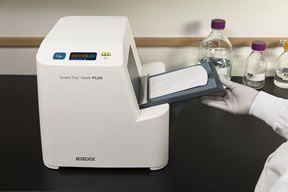
\includegraphics{Step1.jpg}
\caption{add caption -- pictures from our lab...}
\end{figure}

\NP Label bottle with location (geographic area name and stream or lake name),
date, time, water temperature and sampler's initials. Label bottle before
immersion using a black permanent marker or pre-printed labels. QVIR
Bacteria Lab, State Certified Lab, purchases only certified sterile, 100 ml,
sealed containers from IDEXX.

\begin{figure}
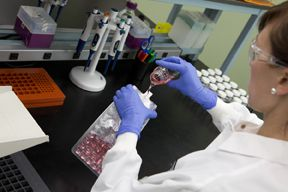
\includegraphics{Step2.jpg}
\caption{add caption -- pictures from our lab...}
\end{figure}


\NP Use latex gloves when handling bottles during sampling. Fingers contain
contaminants such as nitrates. Bug repellents or sunscreen are particularly troublesome as contaminants. Once the gloves are on, be careful not to touch
your face, the ground, or anything but the bottles.

\NP The sample should be taken from flowing, not stagnant water, facing
upstream positioned in the thalwag.


\begin{figure}
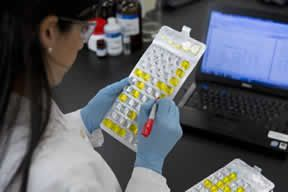
\includegraphics{Step3.jpg}
\caption{add caption -- pictures from our lab...}
\end{figure}

\NP Be sure to immerse the bottle completely, 10 cm (4 inches) deep, with
mouth of bottle pointing upstream, so no water flows over your hand into the
bottle. Be sure the bottle does not get near the bottom of the stream where
sediments can be disturbed. Water samples should be collected 6-12 inches
below the water surface. Fill bottle, to the 100ml line indicated, on first
immersion, pour off the excess and cap. Do not under fill or over fill, do not
redunk. If too much water is poured off, redo sample with new 100 ml
container.

\NP Do not touch bottle mouth or inside of cap. Be careful not to
contaminate the sample with surface film, contact with human skin, breathing
in/on the bottle or cap, etc. If stream is too shallow to immerse bottle fully,
collect as much as possible, being very careful not to touch the bottom. Note
depth on field notes.

\NP Collect one "duplicate" sample every two weeks (sampling frequency).
Sample sites chosen for duplicate sampling are selected at random among
sites sampled. When a duplicate sample is selected for the site, repeat
procedures as with normal stream samples. The duplicate is the second
sample when two samples are collected. Duplicates document repeatability of
individual sample collections and reproducibility of laboratory results.

\NP Samples are analyzed in the Biogeochemistry Lab. Keep samples cool
while transporting. Store at 4 ºC until analysis, but do not freeze. The
maximum holding time is 6 hours.

\NP For each sample, the location number, bottle numbers used and time
collected will be recorded in the field sample log.

\NP The samples will be kept in the possession of researcher personnel who both
collect and analyze the samples.

\subsection{QA/QC}

\NP Accuracy: Initial analyst demonstration of capability and for each new lot of
Quanti-Tray/2000, analyze the following:

\begin{itemize}

\item Check each new lot of Colilert. Shine the ultraviolet lamp on the media snap packs. If the lot is
fluorescent it will be discarded.

\item Dissolve one packet in 100 ml distilled water. Do not incubate.
Check for fluorescents.

\item Analyze sterile reagent water blank with each batch of samples to
verify that there is a negative result from 24-28 hours

\item Gravimetrically check each new lot of sterile, transparent, nonfluorescing 100-ml vessels to ensure the 100-mL fill line is
accurately represented on the vessel. 

\end{itemize}

\subsection{Disposal}

needs updating...

\NP All materials must be autoclaved prior to disposal and workspaces
thoroughly disinfected.

\NP Dispose of media in accordance with Good Laboratory Practices. ??? need to figure out what this means!

\section{Data Analysis and Calculations}

\NP For each sample analyzed, including quality control samples, record
the number of small and large positive wells and the MPN in the
appropriate places on the bench sheet (see below). Calculate
precision for duplicate analyses using equation 1.

\NP Equation 1. 

\begin{equation}
Precision (as RPD) = \frac{(A – B)*100}{(A + B)/2}
\end{equation}

Where: A = MPN from aliquot A and
 B = MPN from aliquot B 
 
 

\NP The following results should be observed:


\begin{table}
\caption{need to add caption}
		\begin{tabular}{ll}\hline

Organism                &  Result \\ \hline \hline
Escherichia coli        & Yellow wells, fluorescence \\
Klebsiella pneumoniae   & Yellow wells, no fluorescence \\
Pseudomonas aeruginosa  & Clear wells, no fluorescence \\
Method Blank            & Clear wells, no fluorescence \\ \hline
  \end{tabular}
\end{table}


\section{QC/QA Criteria}

\subsection{Data assessment and acceptable criteria}

\NP The analyst should review all data for correctness (e.g., use of MPN table).

\NP Precision values are calculated for pairs of duplicate analyses.

\NP Record the precision values as RPD on the bench sheet.

\NP The desired precision is ± 20% (RPD).

\NP The desired detection limit is 1 MPN/100mL

\NP The completed bench sheet is reviewed by the analyst's supervisor or the
QVIR Lab Director 


\subsection{Corrective actions for out-of-control or unacceptable data}

\NP The results for precision and blank data are compared to the
acceptable values for this analysis; ± 20\% and 1 MPN/100mL,
respectively.

\NP If a precision value exceeds 20\% then the analyst should write in the
comments section of the bench sheet: “These data are associated
with an out-of-control duplicate analysis. The UCL = 20\%.” Note:
“UCL” is the Upper Control Limit (i.e., 20%).

\NP If a blank value exceeds 1 MPN/100mL then the analyst should write
in the comments section of the bench sheet: “These data are
associated with a blank value that exceeds the detection limit of 1
MPN/100mL.”

\NP The samples cannot be reanalyzed because the sample volume will be
depleted after the initial analysis.

\NP  If data are unacceptable for any reason, the analyst should review
their analytical technique prior to conducting this analysis again. 

\section{Trouble Shooting}

TBD!!! 


\section{References}

\NP APHA, AWWA. WEF. (2012) Standard Methods for examination of water and wastewater. 22nd American Public Health Association (Eds.). Washington. 1360 pp. (2014).

\end{document}
